\section{Model of the Coherence Manager}
\label{sec:model:cmgr}
This section presents the model for the coherence manager. Since, like the
cache, it implements the behavior as defined by the coherence protocol across
all memory elements, it is a rather complex automaton.

\begin{figure}[hbt!]
\begin{center}
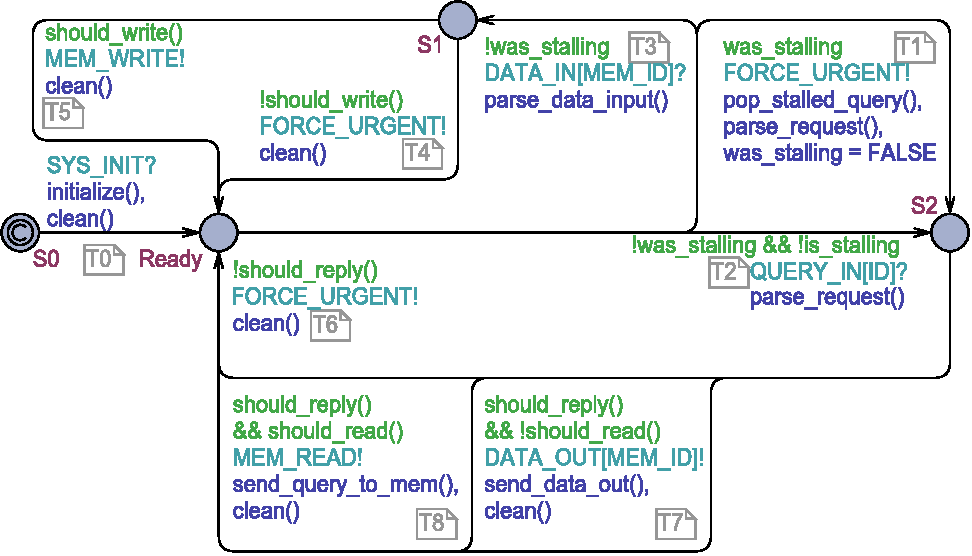
\includegraphics[width=0.7\textwidth]{\chapterdirectory/figure/CoherencyMGR.pdf}
\end{center}
\caption{Automaton for the Coherence Manager}
\label{fig:UPPAAL:CoherencyMGR}
\end{figure}

Figure~\ref{fig:UPPAAL:CoherencyMGR} shows the automaton corresponding to the
coherence manager.

\begin{definition}[Coherence Manager Line Model]
A coherence manager line is defined as $\langle \texttt{addr},\allowbreak{}
\texttt{m\_state}, \texttt{owner} \rangle$ tuple, with \texttt{addr} being the
address of the memory element, \texttt{m\_state} its state in the coherence
manager (including transient states), and \texttt{owner} being the component ID
attributed to it (see \coherencemanagerownerfun{} in
Definition~\ref{def:cmgr_info} from Chapter~\ref{cha:cache_coherence}).
\end{definition}
\begin{example}[Coherence Manager Line Model]
The entry $\langle 93, \text{Shared}, 8\rangle$ would indicate that the memory
element $93$ is considered as \textit{Shared} by the coherence manager, and that
its owner is the component for which the ID is $8$.
\end{example}

As with the caches, the automaton does not directly correspond to the one used
to define the behavior of the coherence manager in the protocol definition, it
is instead reproducing the behavior of that automaton for each memory element.

The coherence manager automaton has the following variables:
\paragraph{Clocks \& Variables for Coherence Manager}
\begin{itemize}
\item
   \lstinline!cache_line_status! is an array of coherence manager lines of
   a size equal to the sum of the size of all caches' \lstinline!cache_lines!
   arrays.
\item
   \lstinline!current_line! is the index of the coherence manager line being
   currently in use.
\item
   \lstinline!stalled_query! is the variable in which a stalled query can be
   put. As indicated in Chapter~\ref{cha:cache_coherence}, the coherence manager
   can \stallact{} queries, but since it is an action taken only after the query
   has been parsed and thus has left its FIFO, it needs a place to remain until
   queries are once again allowed.
\item
   \lstinline!is_stalling! indicates that incoming queries should not be
   handled for now.
\item
   \lstinline!was_stalling! indicates whether the coherence manager just stopped
   stalling and should thus act upon the query stored in
   \lstinline!stalled_query!.
\item
   \lstinline!reply_data_type! indicates the type of data reply that should be
   emitted next.
\item
   \lstinline!should_act_flag! indicates if a data reply should be sent.
\item
   \lstinline!should_mem_flag! indicates if the coherence manager should require
   the memory controller performs an action (either reading or writing).
\end{itemize}
%\end{varandclocks}

The coherence manager's automaton starts in the $S_0$ location.

\paragraph{Transitions for Coherence Manager}
\begin{description}
\item[$S_0 \automatatransitiontrace{T_{0}}{} \texttt{Ready}$]
   Upon synchronization on the \textbf{SYS\_INIT} channel, the coherence manager
   sets its internal variable to sane defaults: all
   \lstinline!cache_line_status! indicate the \textit{Invalid} state, there is
   no \lstinline!stalled_query!, \lstinline!was_stalling! and
   \lstinline!is_stalling! are both \lstinline!false!,
   \lstinline!reply_data_type! is an arbitrary default value,
   \lstinline!should_act_flag! and \lstinline!should_mem_flag! are both set to
   \lstinline!false!.

   The coherence manager is then ready to handle incoming messages.

\item[$\texttt{Ready} \automatatransitiontrace{T_{2}}{} S_2$]
   If the coherence manager is not stalling (\lstinline!is_stalling! set
   to \lstinline!false!) and is not supposed to handle what is stored in
   \lstinline!stalled_query! (\lstinline!was_stalling! set to
   \lstinline!false!), then it may handle incoming queries.

   To retrieve a pending incoming query, the coherence manager synchronizes with
   its query FIFO's dedicated \textbf{QUERY\_IN} sub-channel. This transition
   retrieves the incoming query from the information sharing global variable and
   applies actions according to what is prescribed by the coherence protocol.
   Section~\ref{sec:modeling:cmgr_actions} describes the effect of each actions
   in details.

   Three outcomes are possible: no output is required, a data reply should be
   sent by the coherence manager, or a data reply should be sent by the memory
   controller after reading.

\item[$S_2 \automatatransitiontrace{T_{6}}{} \texttt{Ready}$]
   If no output is required (\lstinline!should_act_flag! is set to
   \lstinline!false!), the coherence manager simply returns to the
   \texttt{Ready} location. It is possible for this transition to have been
   selected because the query lead to a \stallact{}. In such cases, query
   handling has been disabled until the next \resumeact{} action.

\item[$S_2 \automatatransitiontrace{T_{7}}{} \texttt{Ready}$]
   If a data message must be sent, but no \readact{} action was handled, then
   the coherence manager can send the data reply without consulting the memory.
   This corresponds to \lstinline!should_act_flag! set to \lstinline!true! and
   \lstinline!should_mem_flag! set to \lstinline!false!.

   To send a message, the coherence manager sets the information sharing global
   variable so that it contains a data message of the type indicated in
   \lstinline!reply_data_type! for the memory element that is relevant to the
   handled query. Synchronization on the \textbf{DATA\_OUT} sub-channel
   corresponding to the memory controller's ID allows the correct data FIFO to
   handle the outgoing data message.

\item[$S_2 \automatatransitiontrace{T_{8}}{} \texttt{Ready}$]
   If a data message must be sent and a \readact{} action was handled, then
   the coherence manager has to rely on the memory controller to send the data
   message. This corresponds to both \lstinline!should_act_flag! and
   \lstinline!should_mem_flag! set to \lstinline!false! set to \lstinline!true!.

   In this case also, the coherence manager sets the information sharing global
   variable so that it contains a data message of the type indicated in
   \lstinline!reply_data_type! for the memory element that is relevant to the
   handled query. However, the synchronization on the \textbf{MEM\_READ}
   channel, making it one that is also performed by the memory controller's
   automaton and not by a data FIFO. The memory controller will retrieve the
   data message and send it to the data FIFO once the appropriate waiting
   period has elapsed.

\item[$\texttt{Ready} \automatatransitiontrace{T_{3}}{} S_1$]
   Unlike queries, data messages cannot be stalled by the coherence manager.
   Thus, the only reason for the transition that pulls from the incoming data
   messages to not be allowed to fire is if \lstinline!was_stalling! has been
   set to \lstinline!true!. Indeed, if a stalled query has just been un-stalled,
   it is handled before anything else.

   By synchronizing on the \textbf{DATA\_IN} sub-channel corresponding to the
   memory controller's component ID, the oldest pending data message can be
   retrieved from the information sharing global variable. This leads to the
   actions prescribed by the coherence protocol being performed. As with query
   handling, these actions are described in
   Section~\ref{sec:modeling:cmgr_actions}.

   There are two possible outcomes, depending on whether data should be written
   in the main memory or not.

\item[$S_1 \automatatransitiontrace{T_{4}}{} \texttt{Ready}$]
   If there is no need for data to be written (\lstinline!should_mem_flag! set
   to \lstinline!false!), all actions related to the data message have been
   completed, and so the coherence manager simply returns to being able to
   handle the next message.

\item[$S_1 \automatatransitiontrace{T_{5}}{} \texttt{Ready}$]
   If there is a need for data to be written (\lstinline!should_mem_flag! set
   to \lstinline!true!), a synchronization on the \textbf{MEM\_WRITE} channel
   ensures that the memory controller stays busy for the approriate amount of
   time. The coherence manager immediately becomes available for the next
   message however.

\item[$\texttt{Ready} \automatatransitiontrace{T_{1}}{} S_1$]
   A special case of ``next message'' is when the handling of a data message
   led to a \resumeact{} action. Indeed, this indicates that, if there is a
   query held in \lstinline!stalled_query!, the coherence manager is now able
   to act on it. The \lstinline!was_stalling! variable being set to
   \lstinline!true!  indicates that the \resumeact{} action has just occured.

   Handling the stalled query is done in the same way as that of a query being
   pulled from the query FIFO: the actions are performed according to what is
   prescribed by the coherence protocol (see
   Section~\ref{sec:modeling:cmgr_actions}). The difference being that, once
   the actions have been performed, \lstinline!stalled_query! is set back to
   its default value, and \lstinline!was_stalling! is set to \lstinline!false!.
\end{description}

\subsection{Modeling Actions}
\label{sec:modeling:cmgr_actions}
\begin{itemize}
\item \textbf{Stalling:}
   The query is stored in \lstinline!stalled_query! and the
   \lstinline!is_stalling! variable is set to \lstinline!true!. The query will
   only be processed upon a \resumeact{} action for the relevant memory element.
   No other query will be considered in the meantime.

\item \textbf{Changing state:}
   The \lstinline!m_state! field of \lstinline!cache_line_status[current_line]!
   is set to the new value.

\item \textbf{Preparing a data reply:}
   The value of \lstinline!reply_data_type! is set to the requested data type,
   and \lstinline!should_act_flag! is set to \lstinline!true! in order to
   indicate that a data reply ought to be sent.

\item \textbf{Memorizing the current owner:}
   The \lstinline!owner! field of \lstinline!cache_line_status[current_line]!
   is set to the component ID of the sender of the message that led to this
   action being taken. The special component ID \lstinline!NULL! is used if this
   field is to be reset.

\item \textbf{Reading and Writing:}
   It is assumed that reading and writing never both occur as the result of the
   same message: queries can lead to a \readact{}, and data messages can lead
   to a \writeact{}. Thus, setting \lstinline!should_mem_flag! to
   \lstinline!true! indicates that a synchronization with the memory controller
   should be performed as soon as possible. The type of synchronization
   performed depends on whether this was a query or a data message.
\end{itemize}
